\chapter{Metódy}

Pre dosiahnutie rozšírenej reality je potrebné rozoznať, na ktoré miesto v obraze sa má vykresliť daný virtuálny objekt. Tiež treba správne rozhodnúť, aký má byť tento objekt veľký a ako má byť natočený. Na toto rozhodnutie je treba poznať vzájomnú polohu virtuálneho objektu a kamery, respektíve očí používateľa.

Na riešenie problému sa obvykle používajú metódy počítačového videnia. Na ich aplikáciu je potrebné zariadenie s digitálnou kamerou, ktorej záznam softvér analyzuje.

Inou možnosťou je získať informáciu o polohe a smere zorného poľa pomocou iných senzorov. Tento prístup sa dnes používa, ale vymyká sa pôvodnej Azumovej definícii rozšírenej reality \cite{Azuma97} (pozri článok 1.1).

\section{Rozpoznávanie pomocou markerov}

Najjednoduchší spôsob, ako sa dá tento prístup implementovať, je za pomoci markerov. Markery sú obvykle jednoduché asymetrické čiernobiele značky, ktoré sa umiestnia do skutočného sveta tak, aby boli vždy v zábere kamery. Je potrebné zaznačiť, aká je presná poloha, na ktorú sa má vykresliť virtuálny objekt voči tomuto statickému markeru. Občas sa vykresluje priamo na marker, ale obvyklejšie je umiestniť marker len niekam do pozadia. Softvér s rozšírenou realitou potom hľadá vo videu tento marker a keď ho odhalí, tak nájde transformáciu, ktorá marker posunie, otočí a zoškáluje do veľkosti ako je vo videu. Touto transformáciou sa potom transformuje aj virtuálny model, ktorý sa vzápätí vykreslí buď späť do videa, alebo zvlášť na priehľadný displej.

Technológia má presnosť umiestňovania jednotlivých objektov závislú od kvality snímaného obrazu. Vyskytujú sa však chyby, kedy aplikácia pre zlú viditeľnosť nerozozná marker a nič nevykreslí, alebo rozozná za marker skutočný objekt, ktorý markerom nie je a vykreslí virtuálny objekt aj keď ho vykresliť nemá. Ďalšiou nevýhodou je samozrejme to, že v momente, keď sa stratí marker zo záberu, prestane sa vykreslovať aj k nemu prislúchajúci objekt. Tento problém sa dá riešiť buď inštalovaním siete markerov do pozadia, ktoré v sebe majú zakódované svoje súradnice, alebo sledovaním (\emph{trackovaním}) pohybu kamery\footnote{Dá sa namerať priamo z optického toku dát, pomocou informácií z gyroskopu, akcelerometra, magnetometra, alebo ich kombinácie.}. Softvéru potom stačí, aby bol v zábere kamery dobre viditeľný vždy aspoň jeden. Pokiaľ markery neznehodnotia scénu a vývojári potrebujú maximalizovať šance systému na správnu registráciu, môžu sa rozhodnúť použiť pole markerov (po anglicky \emph{marker field}), ktoré pokrýva kompletný povrch scény.

\subsection{Algoritmus rozpoznávania markerov}

Hľadanie markerov sa zvykne robiť nasledovným postupom, ktorý sa zvlášť aplikuje na~každý snímok z kamery. Snímok najprv prejde prahovaním, čo znamená, že sa zmení na binárny. Určí sa istý prah jasu a každý bod obrázku, ktorý má vyšší jas sa prefarbí na biely a všetky ostatné sa prefarbia na čierne. Výsledkom je binárny obraz. Ak sa prah nastaví správne malo by byť v tomto obraze jasne vidno aspoň jeden čiernobiely marker na jednofarebnom pozadí \cite{Kato99}.

Ako ďalší krok sa označia jednotlivé jednofarebné komponenty a~zdetegujú sa ich kontúry. Kontúry sa rozdelia na úsečky a softvér medzi nimi označí priesečníky. Tie, ktoré sú blízko pri sebe a súčet uhlov medzi nimi je blízky 180 stupňom sa odignorujú, pretože tvoria takmer rovnú čiaru a výrazne nemenia tvar objektu. Komponenty, ktoré nemajú štyri ostré vrcholy sa vyradia, pretože nemajú štvorcový tvar. Zvyšné komponenty ostanú kandidátmi na markery. Algoritmus ďalej nájde všetky možné homografie, ktoré zobrazia rohy štvorca na rohy týchto komponentov. Výsledkom sú rotačné matice, ktorými sa transformujú uložené obrázky markerov. Týchto markerov môže byť viac, napríklad ak chce program zobrazovať rôzne objekty na rôzne markery. Po tom, čo sa pre každý komponent vypočítajú cez všetky jeho matice všetky markery z pamäte, sa tieto výsledné obrázky prekryjú s originálnym snímkom a porovnajú \cite{ARToolKit-a}. Binárny obrázok s komponentmi už ďalej nie je potrebný. Pri porovnávaní originálneho snímku s pretransformovaným markerom sa použije niektorá z metód hodnotenia podobnosti. Napríklad sa pre každý pixel vypočíta hodnota rozdielu jasu a potom sa urobí suma všetkých týchto hodnôt. Čím je výsledná hodnota nižšia, tým sú si obrázky podobnejšie.

Pre každého kandidáta na marker sa vyberie ten obrázok, ktorý je mu najpodobnejší a zapamätá sa akou konkrétnou homografiou vznikol. Ak je podobnosť nižšia ako istá hranica, kandidát sa vymaže z výberu a považuje sa za chybu. Výsledkom je zoznam jednotlivých kandidátov, ich súradníc v rámci snímky, k nim prislúchajúce identifikácie markerov (ak sa v aplikácí používa viac markerov) a homografie, určujúce ako na ne niečo premietnuť.

V prípade, že je snahou umiestniť virtuálny objekt priamo na marker, môže sa na~jeho 3D model použiť daná homografia, čím sa správne umiestni, naškáluje a zrotuje, a~vykreslí buď do pôvodného snímku, alebo na priehľadný displej. Ak je marker posunutý, považuje sa za počiatok súradnicovej sústavy a virtuálny objekt sa adekvátne posunie.

Marker samozrejme nemusí byť čiernobiely ani štvorcový, v týchto prípadoch sa algoritmus príslušne upraví. Nakoľko vypočítavanie celého tohoto postupu pre každý snímok v reálnom čase môže byť náročné, často sa využívajú techniky sledovania pohybu. To znamená, že si program pamätá pre objekt jednotlivé polohy a homografie z predchádzajúcich snímkov a prednostne ich vyskúša. Taktiež môže pri plynulom pohybe predpovedať lokácie na nasledovných snímkoch.

Kroky tohoto algoritmu sú znázornené na obrázku \ref{artoolkit}.

\begin{figure}[h]
 \centering
 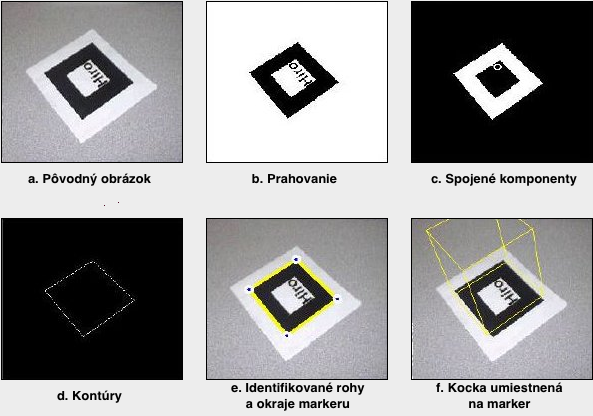
\includegraphics[max width=\textwidth]{pictures/artoolkit.png}
 \caption{Jednotlivé kroky aplikované pri rozpoznávaní markeru, tak ako sú uvedené v dokumentácií knižnice ARToolKit \cite{ARToolKit-a}}
 \label{artoolkit}
\end{figure}

Implementáciu tohoto algoritmu v knižnici ARToolKit využívame aj v demo aplikácii vytvorenej v rámci tejto práce.

\section{Rozpoznávanie na základe významných bodov}

V prípade, že nie je žiadúce použitie markeru, pretože nie je možné modifikovať prostredie, prípadne je potrebné, aby aplikácia fungovala aj v prostrediach, ktoré na tento účel neboli predpripravené, je potrebné túto úlohu riešiť zložitejšiou analýzou. Pri riešení týmto spôsobom musí byť známe ako vyzerá okolie, do ktorého je žiadané vykresliť virtuálny objekt. Toto okolie je potom potrebné rozoznávať v zábere kamery. Táto metóda sa obvykle používa na aplikácie, ktoré napríklad dopisujú v galérií údaje k~obrazom a podobne. V tomto prípade slúži obraz ako špeciálny marker.

\subsection{Rozpoznávanie algoritmom SIFT}
\emph{Scale-invariant feature transform}, alebo SIFT je algoritmus na rozpoznávanie a popisovanie významných bodov vyvinutý Davidom Lowe. Idea je, že objekt, ktorý chceme rozoznávať obsahuje významné body, ktoré sa dajú popísať. Výsledkom je deskriptor, s pomocou ktorého sa dá tento objekt
lokalizovať na iných obrázkoch.

Algoritmus generuje z obrazu objektu množstvo vektorov významných bodov. Tieto vektory sú invariantné na rotáciu a škálovanie obrazu. Významné body obvykle ležia na rohoch, hranách a iných kontrastných miestach, vďaka čomu sú dobre viditeľné aj za~zhoršených podmienok. Pri detekcii sa potom vyhľadáva v tejto databáze významných bodov \cite{Lowe99, Volosin11}.

Jednou z výhod algoritmu SIFT je, že dokáže rozpoznávať aj objekty, ktoré sú čiastočne zakryté. Jedným z následníkov SIFT je napríklad SURF (celý názov \emph{Speeded Up Robust Features}), ktorý je približne osem krát rýchlejší. SURF je
patentovaný Herbertom Bayom \cite{Bay06}. Ďalšími algoritmami na rozpoznávanie významných bodov sú BRIEF \cite{Calonder10} (\emph{Binary Robust Independent Elementary Features}), ktorý má podobné alebo lepšie výsledky ako SURF, BRISK (\emph{Binary Robust Invariant Scalable
Keypoints}) \cite{Leutenegger11}, FREAK (\emph{Fast Retina Keypoint}) \cite{Alahi12}, SUSSAN \cite{Smith97}, FAST \cite{Tuzel06} a DAISY \cite{Tola10}.

\section{Rozpoznávanie na základe GPS}

V prípade, že sú známe presné polohy virtuálnych objektov a nie je známe ako vyzerá okolie, do ktorého sa majú tieto objekty vykresliť, ako napríklad pri aplikáciach, čo do reálneho sveta dokreslujú mapu okolia, názvy firiem a podobne, problém sa rieši pomocou GPS. Tieto aplikácie majú databázu, v ktorej majú pri všetkých údajoch obsiahnuté aj súradnice GPS. Používateľ potom potrebuje zariadenie s GPS a digitálnym kompasom, ktoré na základe dát z GPS a kompasu vypočíta, na ktorý objekt v databáze je namierená kamera, alebo hlava používateľa, kde by sa tento objekt mal nachádzať v zábere a pod akým uhľom a v akej veľkosti ho má byť vidno \cite{Bimber05}.

Aby aplikácia spĺňala Azumovu definíciu rozšírenej reality, je túto metódu potrebné skombinovať s metódami rozpoznávania obrazu. V praxi však existujú aj aplikácie, ktoré sa spoliehajú čisto na dáta z GPS a v prípade použitia zariadenia s priehľadným displejom, kameru ignorujú, pretože žiadnu analýzu obrazu nevykonávajú. Táto metóda je všeobecne menej presná ako metódy rozpoznávania obrazu, pretože používané senzory obvykle nie sú také presné a virtuálne objekty sa teda nemusia vykresliť presne na to správne miesto a môžu byť posunuté. Malou výhodou techniky je, že by sa pri~jej používaní nemali vyskytovať chyby, kedy nevykreslíme objekt (napríklad ako pri nerozoznanom markeri), prípadne chyby, pri ktorých sa vykreslí objekt na miesto, na ktoré sa žiaden objekt vykresliť nemá.

\section{Prehľad softvérových knižníc }

Existuje niekoľko softvérových knižníc uľahčujúcich implementáciu aplikácií vytvárajúcich rozšírenú realitu.

Jednou z prvých takýchto knižníc je ARToolKit vyvinutý Hirokazu Katom v roku 1999 pre jazyky C a C++. Táto knižnica deteguje markery a prepočítava pod~akým uhlom ich používateľ vidí. Vývojárom ďalej poskytuje súradnicový systém, ktorý do tohoto priestoru transformuje. ARToolKit je k dispozícií zadarmo pod licenciou GNU/GPL \cite{ARToolKit-b}. Z tejto knižnice vychádza množstvo ďalších nasledovníkov a dodnes sa používa. Využívame ju za účelom registrácie objektov v aplikácii s~rozšírenou realitou, ktorá je súčasťou tejto práce.

ARToolkitPlus bol otvorený tracker, ktorý vychádzal z ARToolKitu. Jeho vývoj sa zastavil v roku 2007 a bol nahradený Studierstube trackerom, ktorý už však nie je verejne prístupný \cite{Wagner07}.

Studierstube je framework vyvinutý na \emph{Graz University of Technology}. Na trackovanie sa odporúča použiť OpenTracker od rovnakých autorov. Vývoj bol ukončený v~roku 2008 \cite{Studierstube-a, Studierstube-b}.

ArUco je minimalistická knižnica pre C++. Rozpoznáva markery, alebo polia markerov a je veľmi rýchla vďaka tomu, že sa opiera o OpenCV \cite{ArUco}.

Vuforia je proprietárnou knižnicou, ktorá dokáže rozpoznávať obrázky a jednoduché 3D objekty. Dá sa používať v C++, Jave a Objective-C, vďaka čomu je obľúbená na~mobilných platformách iOS a Android \cite{Vuforia}.